\documentclass[pdf, unicode, notheorems, xcolor={table}]{beamer}
\usetheme[numbers, totalnumbers, minimal]{Statmod}

% \documentclass[pdf, 8pt, unicode, xcolor={table}]{beamer}
\usepackage[T2A]{fontenc}
\usepackage[utf8]{inputenc}
\usepackage[russian]{babel}

\beamertemplatenavigationsymbolsempty


\usepackage{multirow}
\usepackage{hhline}
% \usepackage[table]{xcolor}
\usepackage{graphicx}
\usepackage{hyperref}

\usepackage{amssymb}
\usepackage{amsthm}

\usepackage[linesnumbered,ruled]{algorithm2e}

\usefonttheme[onlymath]{serif}

\usepackage{beamerthemesplit}

\addtobeamertemplate{navigation symbols}{}{%
	\usebeamerfont{footline}%
	\usebeamercolor[fg]{footline}%
	\hspace{1em}%
	\insertframenumber/\inserttotalframenumber
}

\setbeamerfont{institute}{size=\normalsize}

\setbeamercolor{bluetext_color}{fg=blue}
\newcommand{\bluetext}[1]{{\usebeamercolor[fg]{bluetext_color}#1}}
\def\R{{\normalfont\ttfamily R}}
\newcommand{\code}[1]{\texttt{#1}}
\DeclareMathOperator*{\argmin}{\arg\!\min}

\setbeamercovered{transparent}
\setbeamertemplate{caption}[numbered]

\graphicspath{{fig/}}
%\input{monogr}
%\input{mondef}
%\input{monscrt}

\makeatletter
\newlength\beamerleftmargin
\setlength\beamerleftmargin{\Gm@lmargin}
\makeatother

\title[SSA EOP Time Series Prediction]{Application of Singular Spectrum Analysis \\ for EOP Time Series Prediction}


\author{Okhotnikov Grigory}

\institute{
Saint Petersburg State University \\
Mathematics and Mechanics Faculty \\
Statistical Modelling \\

\vspace{0.5cm}

 Scientific supervisor: Associate Professor {\bf Nina Golyandina}, PhD, SPbU.
 }

 \date{
    Saint Petersburg 2017
}

\begin{document}

\maketitle


\begin{frame}\frametitle{SSA}

We introduce the system for forecasting of the time series of the Earth rotation parameters $ x, y, LOD,  dX, dY $. 

\smallskip
Singular spectrum analysis (SSA) together with cross-validation technique for the choice of the SSA parameters
is used for forecast construction.

\medskip
SSA theory and implementation sources:
	\begin{itemize}
		\item Book ``Analysis of Time Series Structure: SSA and Related
		Techniques'' (Nina Golyandina, Vladimir Nekrutkin, Anatoly Zhigljavsky)
		\item Software: \code{Rssa} package, \code{rforecast} function \\
		{\scriptsize \color{blue}
		(\url{https://github.com/asl/rssa}, \\
		\url{cran.r-project.org/package=Rssa})}
	\end{itemize}
\end{frame}

\begin{frame}\frametitle{Data Sources}
	Source data:
	\begin{itemize}
		\item Bulletin IERS (International Earth rotation and Reference systems Service) C04;
		\\ {\scriptsize \color{blue}
		(\url{http://hpiers.obspm.fr/iers/eop/eopc04/eopc04_IAU2000.62-now})}
		\item finals2000A.daily file is used to fill gaps of Bulletin C04 (latest 30 days).
		\\ {\scriptsize \color{blue}  (\url{https://datacenter.iers.org/eop/-/somos/5Rgv/latest/13})}
	\end{itemize}

	\vspace{0.5cm}

	Forecasts to compare with:
	\begin{itemize}
		\item Pul AM~--- Pulkovo EOP and Reference Systems Analysis Center forecasts (LS + ARIMA); {\scriptsize \color{blue} (\url{http://www.gao.spb.ru/english/as/persac/eopcppp/})}
		\item Bull A~--- Bulletin IERS A forecasts. {\scriptsize \color{blue} (\url{https://datacenter.iers.org/eop/-/somos/5Rgv/latest/6})}
	\end{itemize}
\end{frame}

\begin{frame}\frametitle{Forecasts Comparison}
	Comparison table of mean squared errors of forecasts from different sources for 50 days taken from each year of 2011, 2012, 2013, 2014, 2015 spaced at intervals of 7 days starting from January 1 (250 days in total).
	\begin{table}[!hhh]
		\centering
		\small
		\begin{tabular}{|c|c|c|c|}
			\hline
			& SSA & Pulkovo AM & Bulletin A \\
			\hline
			$ x $   & \cellcolor{blue!25} $ 7.2 \times 10^{-4} $ & $ 8.6 \times 10^{-4} $ & $ 7.5 \times 10^{-4} $  \\
			\hline
			$ y $   & \cellcolor{blue!25} $ 6.1 \times 10^{-4} $ & $ 7.6 \times 10^{-4} $ & $ 8.5 \times 10^{-4} $ \\
			\hline
			$ LOD $ & \cellcolor{blue!25} $ 9.1 \times 10^{-8} $ & $ 1.0 \times 10^{-7} $ &  \\
			\hline
			$ dX $  & $ 1.3 \times 10^{-8} $ & \cellcolor{blue!25} $ 1.1 \times 10^{-8} $ &  \\
			\hline
			$ dY $  & \cellcolor{blue!25} $ 1.6 \times 10^{-8} $ & $ 2.2 \times 10^{-8} $ &  \\
			\hline
		\end{tabular}
	\end{table}

	The proposed SSA method performs better on average than other techniques for $ x, y $ and $ LOD $ time series. Forecasts of $ dX $ and $ dY $ time series are comparable with forecasts of Pulkovo observatory.
\end{frame}


\begin{frame}\frametitle{Tab: Forecasts for 365 Days}
	\begin{figure}
		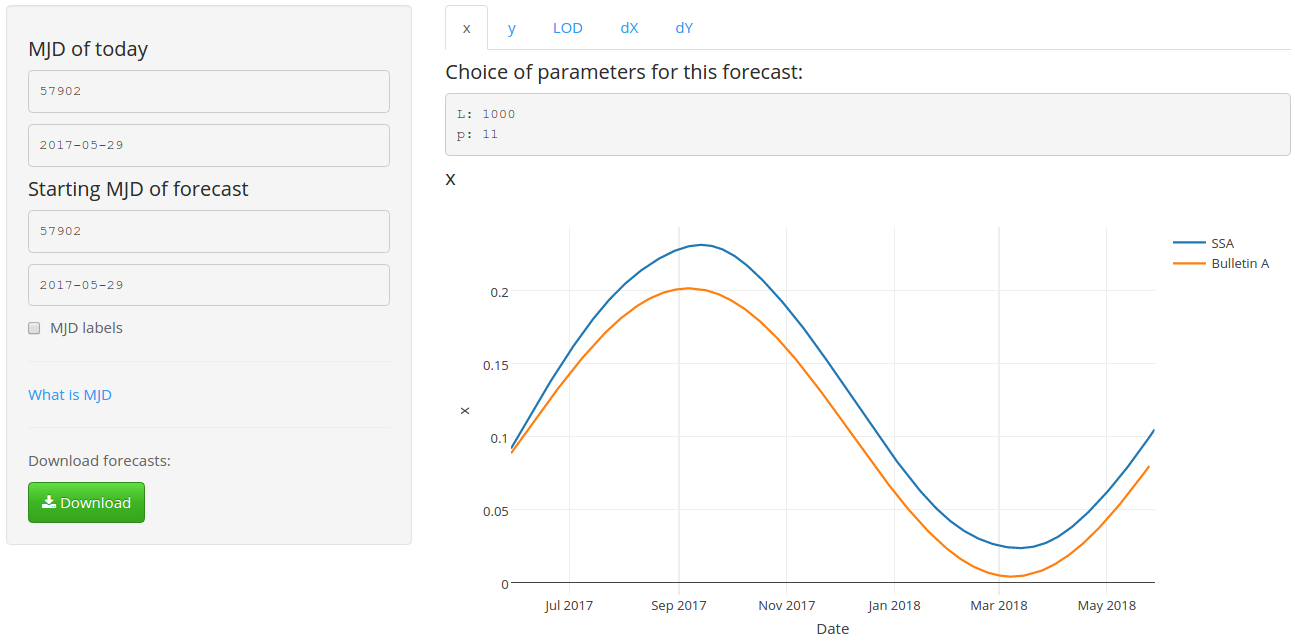
\includegraphics[width=0.9 \linewidth]{forecast_365}
	\end{figure}
	\begin{itemize}
		\item SSA forecasts of each EOP time series \textbf{for 365 days} is available on the first page.
		\item SSA forecasts are performed from the current date.
		\item SSA forecast: blue line, Bulletin A forecast: yellow line.
		\item SSA forecasts are generated automatically using time-series cross-validation technique for choosing the parameters.
	\end{itemize}
\end{frame}

\begin{frame}\frametitle{Tab: Forecasts for 365 Days}
	\begin{itemize}
	\item Use tab switcher to view plots of forecasts for other time series.
	\item All forecasts can be downloaded as one file using button `Download'.
	\end{itemize}
	\begin{figure}
		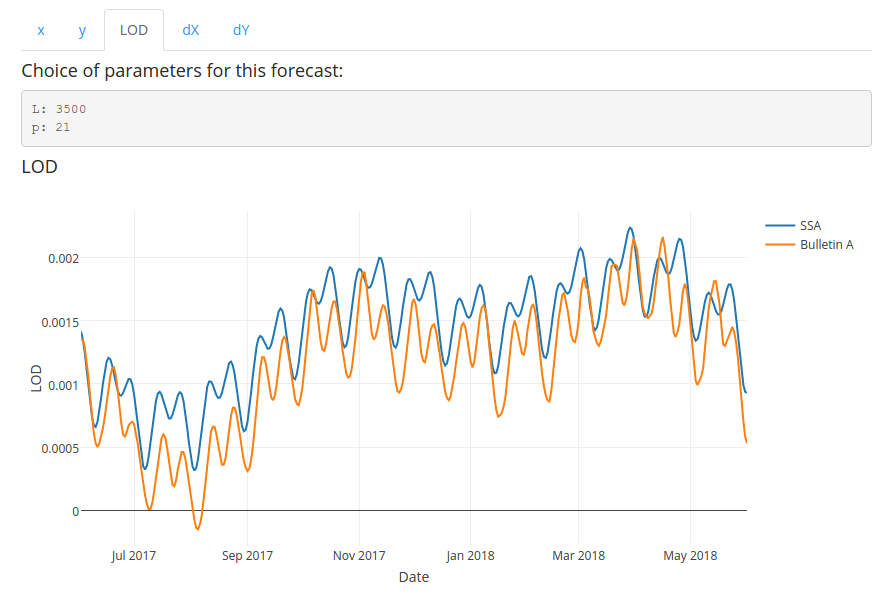
\includegraphics[width=0.9 \linewidth]{tab_lod}
	\end{figure}
\end{frame}

\begin{frame}\frametitle{Tab: Forecasts for 365 Days}
	\begin{figure}
		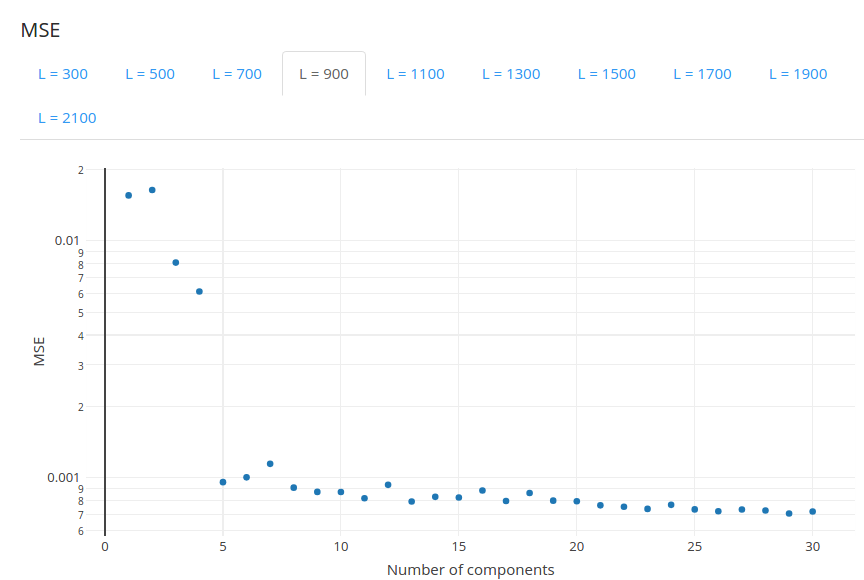
\includegraphics[width=0.8 \linewidth]{mse}
	\end{figure}

	Mean squared error (MSE) of forecasts at different values of $L$ and number of components $r$ are reported below. This information can be used when generating the forecasts manually.
\end{frame}

\begin{frame}\frametitle{Tab: Generate Forecast}
	\begin{minipage}[t]{0.48\linewidth}
		\begin{figure}
			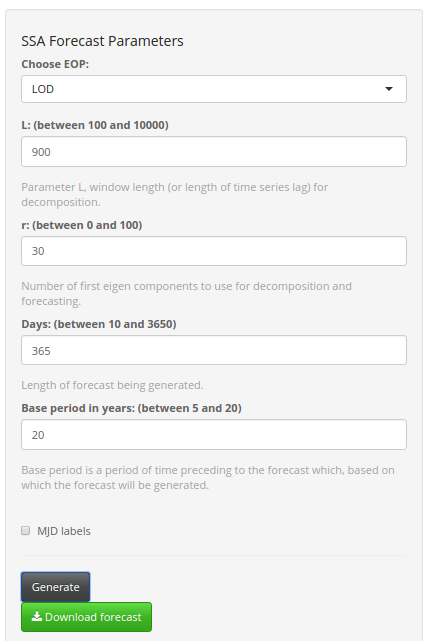
\includegraphics[width=\linewidth]{generate_params}
		\end{figure}
	\end{minipage}%
	\hfill%
	\begin{minipage}[t]{0.48\linewidth}
		\begin{itemize}
		\item This page offers an interface for the manual forecast generation with the given forecast horizon (in days).

		\item SSA forecasts are performed from the current date.

		\item SSA parameters can be specified using panel on the left side of the page.
		
		\item Generated forecasts can be downloaded by clicking `Download forecast' button.
		\end{itemize}
	\end{minipage}
\end{frame}

\begin{frame}\frametitle{Tab: Generate Forecast}
	\begin{figure}
		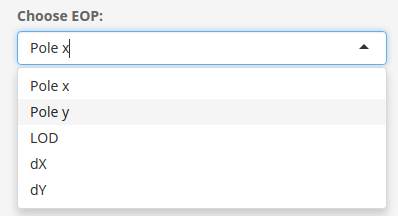
\includegraphics[width=0.9 \linewidth]{dropdown}
	\end{figure}
	At first, choose the time series to predict.
\end{frame}

\begin{frame}\frametitle{Tab: Generate Forecast}
	\begin{figure}
		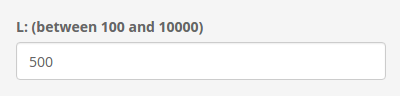
\includegraphics[width=0.9 \linewidth]{parameter_L}
	\end{figure}
	Then specify the value of the parameter $ L $ (the window length).
	
	There is no exact formula for the ``best'' value. To choose $L$, you can look at MSE of forecasts on Tab `Forecasts for 365 Days'.
\end{frame}

\begin{frame}\frametitle{Tab: Generate Forecast}
	\begin{figure}
		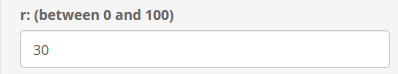
\includegraphics[width=0.9 \linewidth]{parameter_r}
	\end{figure}
	Specify the value of the parameter $ r $ (the number of elementary components used for reconstruction).
	
	Typically, this value is not larger than 30 for $ x, y, LOD $ series and not larger than 5 for $ dX $ and $ dY $.
\end{frame}

\begin{frame}\frametitle{Tab: Generate Forecast}
	\begin{figure}
		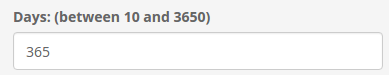
\includegraphics[width=0.9 \linewidth]{number_of_days}
	\end{figure}
	Set the length of the forecast (forecasting horizon) in days.
	
	\begin{figure}
		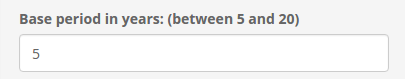
\includegraphics[width=0.9 \linewidth]{base_period}
	\end{figure}
	Define how many latest values should be used as the base for reconstruction and forecasting.
	
\end{frame}

\begin{frame}\frametitle{Tab: Generate Forecast}
	\begin{figure}
		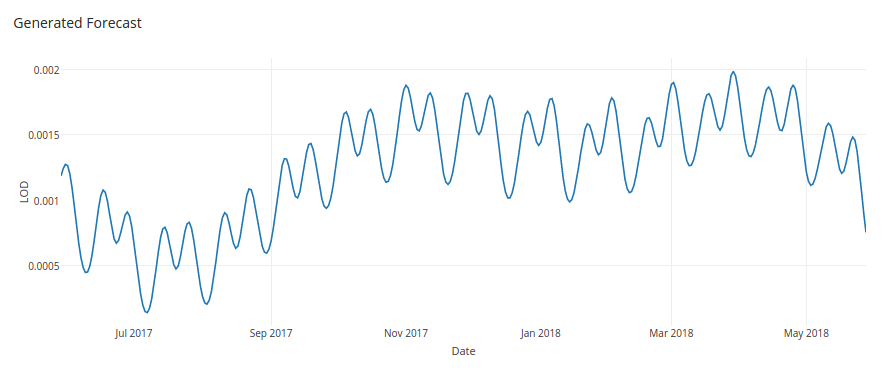
\includegraphics[width=0.8 \linewidth]{generate_result}
	\end{figure}
	Resulting forecast can look like this.
\end{frame}

\begin{frame}\frametitle{Tab: Compare Forecasts}
	\begin{figure}
		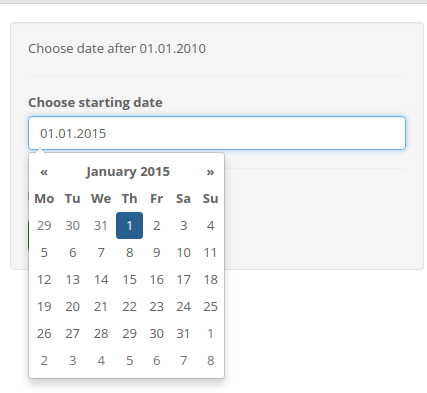
\includegraphics[width=0.4 \linewidth]{compare_date}
	\end{figure}
	Forecasts generated by the proposed method can be compared with forecasts from other sources for any arbitrary day in the past.
	
	Use the `date input' field to specify the date to compare 365 days forecasts starting from this day.
\end{frame}

\begin{frame}\frametitle{Tab: Compare Forecasts}
	\begin{figure}
		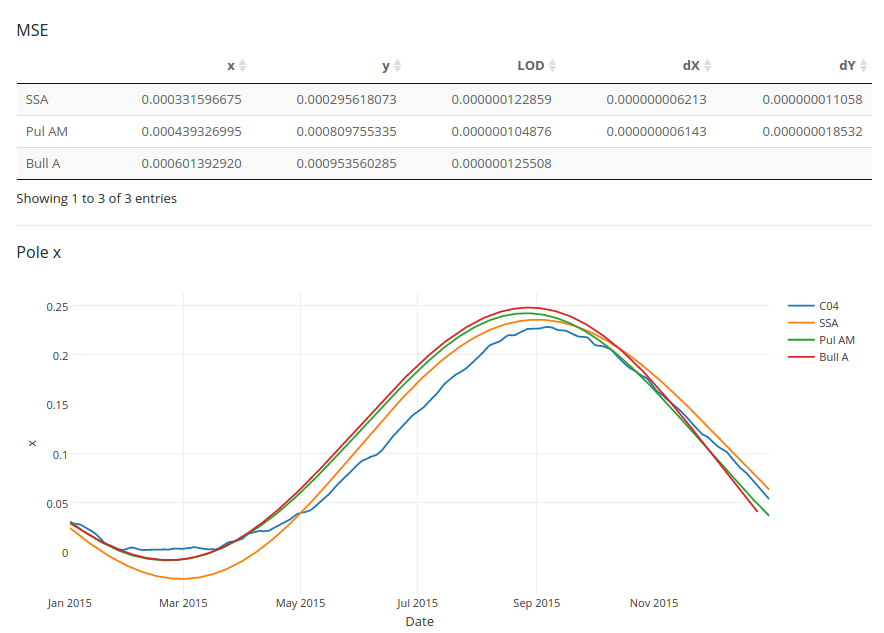
\includegraphics[width=0.7 \linewidth]{compare_result}
	\end{figure}
	MSE comparison table and plots of different forecasts are reported on the main part of the page.
	
	MSE values can be sorted by ascending or descending order by clicking on the column header of interest.
\end{frame}


\end{document}
